%\documentclass[manuscript]{acmart}
%\documentclass[acmsmall]{acmart}
%\settopmatter{printacmref=false}


\documentclass[
  a4paper,
  12pt,
  DIV=12,        % höherer Wert = schmalere Ränder, weniger Whitespacmi
  parskip=half,  % Absätze mit halbem Abstand statt Einzug
  headings=small % kleinere Überschriften, weniger vertikaler Abstand
]{scrartcl}

%\documentclass[a4paper,11pt]{scrartcl}
%\documentclass[a4paper,11pt]{report}
%\documentclass[a4paper,12pt]{book}
\usepackage[utf8]{inputenc}
\usepackage[german]{babel}
\usepackage[T1]{fontenc}
\usepackage{lmodern}
\usepackage{graphicx}
\usepackage{amsmath}
\usepackage{caption}
\usepackage{gensymb}
\usepackage{microtype}
\usepackage{longtable}
\usepackage{tabularx}   % Spalten, die die restliche Zeilenbreite auffüllen (X-Spalte)
\usepackage{booktabs}   % \toprule \midrule \bottomrule (in mobrob_table.tex verwendet)
\usepackage{wrapfig}    % Textumfluss um Abbildungen
\usepackage{array}
\usepackage{calc}

\usepackage[citecolor=black, colorlinks=true, linkcolor=black, urlcolor=blue]{hyperref}


%\usepackage{geometry}
\usepackage{siunitx}
%\geometry{margin=2.5cm}


\usepackage{amsthm}
\usepackage{mdframed}
\usepackage{enumitem}

\newmdtheoremenv{theorem}{Theorem}

\theoremstyle{definition}
\newmdtheoremenv{derivation}{Derivation}

\providecommand{\tightlist}{%
  \setlength{\itemsep}{0pt}\setlength{\parskip}{0pt}}

%\mdfdefinestyle{leftline}{
%    topline=false, bottomline=false, rightline=false,
%    linewidth=2pt, linecolor=gray
%}
\theoremstyle{definition}
\newmdtheoremenv[style=leftline]{myalgorithm}{Algorithm}




%\usepackage{fancyvrb}







\let\Bbbk\relax
\usepackage{amssymb}


\usepackage{yfonts}

\usepackage{kvmap}

\usepackage[
    backend=biber,
    style=alphabetic,
    sortlocale=de_DE,
    natbib=true,
    %url=false,
    doi=true,
    %eprint=false
]{biblatex}
\addbibresource{literatur.bib}

%\usepackage[
%    backend=biber,
%    style=alphabetic,
%    sortlocale=de_DE,
%    natbib=true,
%    %url=false,
%    doi=true,
%    %eprint=false
%]{biblatex}
%\addbibresource{Literaturrecherche-Dennis/mobrob_references.bib}

\usepackage[autostyle=true,german=quotes]{csquotes}
\usepackage{trfsigns} %fourier transform arrow
\usepackage{mathrsfs} %fourier F
\usepackage{commath}

\usepackage{pgfplots}
\pgfplotsset{compat=1.18}

\usepackage{xcolor}
\usepackage{listings}
\usepackage[european]{circuitikz}
\ctikzset{tripoles/european not symbol=ieee circle}

%\usepackage[shading]{moeptikz}
%\moeptikzset{shading=true}

%\usepackage{german,longtable}

\usepackage{xcolor}
\usepackage{color}
\usepackage{url}

\usepackage{xfrac}

\usepackage{listings}
\usepackage{verbatimbox}

\usepackage{algorithm}
\usepackage{algpseudocode}

\usepackage{multirow}
\usepackage{float}
\usepackage{pdflscape}   % einzelne Querformatseiten (im PDF gedreht)

%%%% TIKZ

\usepackage{tikz}

\usepackage{pgfplots}
\usetikzlibrary{calc,
trees,positioning,arrows,
chains,shapes.geometric,
decorations.pathreplacing,
decorations.pathmorphing,shapes,
matrix,shapes.symbols,
plotmarks}
%\tikzexternalize[prefix=figures/]

%\tikzset{%
%  block/.style    = {draw, thick, rectangle, minimum height = 3em,
%    minimum width = 3em},
%  sum/.style      = {draw, circle, node distance = 2cm}, % Adder
%  input/.style    = {coordinate}, % Input
%  output/.style   = {coordinate} % Output
%}
% Defining string as labels of certain blocks.
%\newcommand{\suma}{\Large$+$}
%\newcommand{\multa}{\Large$\times$}
%\newcommand{\inte}{$\displaystyle \int$}
%\newcommand{\derv}{\huge$\frac{d}{dt}$}

\usetikzlibrary{arrows,automata,positioning}
%\usepackage{automata}


%%% END TIKZ

\usepackage[section]{placeins}

\usepackage{textcomp}


\usepackage{listings}
\usepackage{verbatimbox}

\usepackage{bold-extra}

\usepackage{framed}

%\usepackage{fancyhdr}
%\pagestyle{fancy}
%\lhead{\leftmark}
%\chead{}
%\rhead{}
%\lfoot{}
%\cfoot{\thepage}
%\rfoot{}
%\renewcommand{\headrulewidth}{0.2pt}
%\renewcommand{\footrulewidth}{0.2pt}



\newcommand{\Z}{\mathbb{Z}}
\newcommand{\R}{\mathbb{R}}
\newcommand{\C}{\mathbb{C}}
\newcommand{\N}{\mathbb{N}}
\newcommand{\SqrtNy}{$\sqrt{\textsc{Ny}}$}
\newcommand{\conj}{\overline}
\newcommand{\Kset}{\textswab{K}}
\newcommand{\Qset}{\textswab{Q}}
\newcommand{\ceil}[1]{\left\lceil #1 \right\rceil}
\newcommand{\floor}[1]{\left\lfloor #1 \right\rfloor}
\newcommand{\sorted}[1]{\textsc{sort}\left\lbrace #1 \right\rbrace}
\newcommand{\SNRgain}{a_{SNR}}
\newcommand{\EQgain}{a_{EQ}}
\newcommand{\SIRgain}{a_{SIR}}
\newcommand{\SNIRgain}{a_{SINR}}
\newcommand{\SNR}{\textsc{SNR}}
\newcommand{\CIRgain}{a_{CIR}}
\newcommand{\CINRgain}{a_{CINR}}
\newcommand{\CNR}{\textsc{CNR}}
\newcommand{\CINR}{\textsc{CINR}}
\newcommand{\HPAModel}{ Hughes 1177H TWTA }
\newcommand{\bigO}{\mathcal{O}}
\newcommand{\CopWinCompl}{2.375377}
\newcommand{\IBO}{\textsc{IBO}}
\newcommand{\OBO}{\textsc{OBO}}
\newcommand{\spacepage}{\newpage\null\thispagestyle{empty}\newpage}
\newcommand{\satcom}{ SatCom }
\newcommand{\db}{~\text{dB}}


\definecolor{mGreen}{rgb}{0,0.6,0}
\definecolor{mGray}{rgb}{0.5,0.5,0.5}
\definecolor{mPurple}{rgb}{0.58,0,0.82}
\definecolor{backgroundColour}{rgb}{0.95,0.95,0.92}

\lstdefinestyle{CStyle}{
    backgroundcolor=\color{backgroundColour},
    commentstyle=\color{mGreen},
    keywordstyle=\color{magenta},
    numberstyle=\tiny\color{mGray},
    stringstyle=\color{mPurple},
    basicstyle=\footnotesize,
    breakatwhitespace=false,
    breaklines=true,
    captionpos=b,
    keepspaces=true,
    numbers=left,
    numbersep=5pt,
    showspaces=false,
    showstringspaces=false,
    showtabs=false,
    tabsize=2,
    language=C
}

\lstdefinelanguage{VHDL}{
  morekeywords=[1]{library,use,all,entity,is,port,in,out,end,architecture,of,begin,process,if,then,else,elsif,when,others,signal,variable,wait,for,loop},
  morecomment=[l]--,
  morestring=[b]",
  sensitive=true
}

\lstset{
  language=VHDL,
  basicstyle=\ttfamily\small,
  keywordstyle=\color{blue},
  commentstyle=\color{gray},
  stringstyle=\color{red},
  numbers=left,
  numberstyle=\tiny,
  stepnumber=1,
  numbersep=8pt,
  frame=single,
  breaklines=true,
  captionpos=b
}

\lstset{numbers=none}

%\newcounter{example}
%\renewcommand{\theexample}{\thesection.\arabic{example}}


% Default fixed font does not support bold face
\DeclareFixedFont{\ttb}{T1}{txtt}{bx}{n}{12} % for bold
\DeclareFixedFont{\ttm}{T1}{txtt}{m}{n}{12}  % for normal

% Custom colors
\usepackage{color}
\definecolor{deepblue}{rgb}{0,0,0.5}
\definecolor{deepred}{rgb}{0.6,0,0}
\definecolor{deepgreen}{rgb}{0,0.5,0}

\usepackage{listings}

% Python style for highlighting
\newcommand\pythonstyle{\lstset{
language=Python,
basicstyle=\ttm,
morekeywords={self},              % Add keywords here
keywordstyle=\ttb\color{deepblue},
emph={MyClass,__init__},          % Custom highlighting
emphstyle=\ttb\color{deepred},    % Custom highlighting style
stringstyle=\color{deepgreen},
frame=tb,                         % Any extra options here
showstringspaces=false
}}


% Python environment
\lstnewenvironment{python}[1][]
{
\pythonstyle
\lstset{#1}
}
{}

% Python for external files
\newcommand\pythonexternal[2][]{{
\pythonstyle
\lstinputlisting[#1]{#2}}}

% Python for inline
\newcommand\pythoninline[1]{{\pythonstyle\lstinline!#1!}}





\nocite{*}


\begin{document}
%\pagenumbering{roman}



\title{Coasterbot}
\subtitle{Aufgabenliste}
\author{Dennis Borutta}
%\email{gereonsuch@suchdsp.com}
%\affiliation{
%  \institution{Wilhelm Büchner University of Applied Sciences}
%  \department{Computer Engineering}
%  \city{Hof}
%  \country{Germany}
%}



\begin{titlepage}
  \begin{center}
    {\large Wilhelm Büchner University of Applied Sciences} \\[0.3em]

    {\normalsize Projektseminar Master}
\vspace{5em}

    {\LARGE\bfseries Coasterbot} \\[0.5em]

    {\large Unternehmensvorstellung} \\[1em]

    {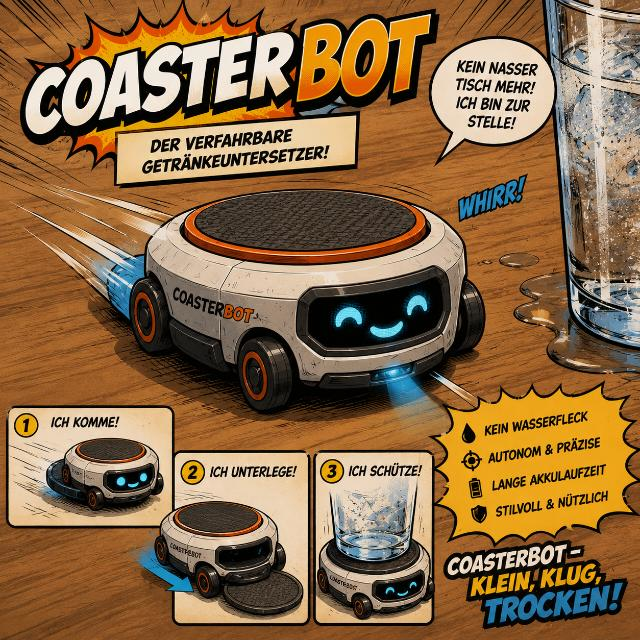
\includegraphics[width=0.38\textwidth]{coasterbot.png}} \\[1em]

\vspace{4em}

    {\normalsize
\begin{tabular}{ll}
Dennis Borutta, B. Eng & dennis.borutta@outlook.com\\
Stefan Etringer, B. Eng & mail@stefan.works\\
Gereon Such, M. Sc. & gereonsuch@gmail.com\\
\end{tabular}
    }
  \end{center}


\end{titlepage}


% einleitung preambel etc.


% Versionshistorie des Dokuments -- eigene Seite direkt nach dem Titelblatt
\section*{Versionshistorie}

\begin{tabularx}{\textwidth}{@{}clp{2.6cm}X@{}}
\toprule
\textbf{Version} & \textbf{Datum} & \textbf{Bearbeiter} & \textbf{Änderungen}\\
\midrule
1 & 15.08.2026 & Borutta & Erstfassung der Aufgabenliste\\
2 & 18.08.2026 & Ertringer, Borutta, Such & Aktualisierung nach Projektbesprechung\\
3 & 25.08.2026 & Ertringer, Borutta, Such & Aktualisierung nach Projektbesprechung\\
\bottomrule
\end{tabularx}


\newpage

\tableofcontents

\newpage

\section{Einleitung}\label{einleitung}

``Eine Aufgabenliste (auch: To-do-Liste, Liste offener Punkte,
Action-Item-Liste) hält fest, welche Aufgaben im Projekt anstehen, bis
wann sie erledigt sein müssen und wer sie verantwortet. Die Einträge
ergeben sich in der Regel aus Besprechungsdokumenten, beispielsweise im
Nachgang der Projekt-Jour-fixes; die Statusverfolgung geschieht meist
ebenfalls im Rahmen der Besprechungen.''\cite{BibEntry2013Sep} Damit verbindet die
Aufgabenliste die Projektplanung mit der Ausführung. In diesem Dokument
wird eine solche Aufgaben liste für die Teilaufgabe `Konzeption
ausarbeiten' ausgearbeitet.

\newpage
\begin{landscape}
\section{Aufgabenliste}\label{aufgabenliste}

Betrachtete Teilaufgabe: Konzeption ausarbeiten

Start: 15.08.2026

Ende: 04.09.2026

{\def\LTcaptype{none} % do not increment counter
\begin{longtable}[]{@{}
  >{\raggedright\arraybackslash}p{0.20\linewidth}
  >{\raggedright\arraybackslash}p{0.13\linewidth}
  >{\raggedright\arraybackslash}p{0.09\linewidth}
  >{\raggedright\arraybackslash}p{0.09\linewidth}
  >{\raggedright\arraybackslash}p{0.08\linewidth}
  >{\raggedright\arraybackslash}p{0.20\linewidth}
  >{\raggedright\arraybackslash}p{0.15\linewidth}
@{}}
\toprule\noalign{}
\begin{minipage}[b]{\linewidth}\raggedright
Aufgabe
\end{minipage} & \begin{minipage}[b]{\linewidth}\raggedright
Verantwortliche Person
\end{minipage} & \begin{minipage}[b]{\linewidth}\raggedright
Termin
\end{minipage} & \begin{minipage}[b]{\linewidth}\raggedright
Status
\end{minipage} & \begin{minipage}[b]{\linewidth}\raggedright
Priorität
\end{minipage} & \begin{minipage}[b]{\linewidth}\raggedright
Abhängigkeiten
\end{minipage} & \begin{minipage}[b]{\linewidth}\raggedright
Arbeitspaket
\end{minipage} \\
\midrule\noalign{}
\endhead
\bottomrule\noalign{}
\endlastfoot
Testfälle aus Lastenheft ableiten & Stefan Etringer & 20.08.2026 &
Erledigt & Mittel & -- & Testfälle definieren \\
Bewertungsmatrizen ausarbeiten & Stefan Etringer & 21.08.2026 & Erledigt
& Hoch & Tesfälle abgeleitet & Testfälle definieren \\
Mögliche Sensorik aus Lastenheft ableiten und auswählen & Gereon Such &
18.08.2026 & Erledigt & Hoch & -- & Sensorik/Aktorik auswählen \\
Mögliche Aktorik aus Lastenheft ableiten und auswählen & Gereon Such &
19.08.2026 & Erledigt & Hoch & -- & Sensorik/Aktorik auswählen \\
Mögliche Energieversorgung und Steuerung ableiten und auswählen & Gereon
Such & 20.08.2026 & Erledigt & Hoch & -- & Sensorik/Aktorik auswählen \\
Elektronikbedarfe in Stückliste aufnehmen & Gereon Such & 21.08.2026 &
Erledigt & Hoch & Elektronikbedarfe definiert & Sensorik/Aktorik
auswählen \\
Mögliche Hardware aus Lastenheft ableiten und auswählen & Dennis Borutta
& 18.08.2026 & Erledigt & Mittel & -- & Sensorik/Aktorik auswählen \\
Modell des Prototypen ausarbeiten & Dennis Borutta & 20.08.2026 &
Erledigt & Hoch & Hardwarelösung ausgewählt & Sensorik/Aktorik
auswählen \\
Mechanikbedarfe in Stückliste aufnehmen & Dennis Borutta & 21.08.2026 &
Erledigt & Hoch & Modell ausgearbeitet & Sensorik/Aktorik auswählen \\
Mögliche Softwarearchitektur aus Lastenheft ableiten & Stefan Etringer &
20.08.2026 & Erledigt & Mittel & Sensorik/Aktorik ist bekannt &
Softwarearchitektur erarbeiten \\
Softwarearchitektur skizzieren & Stefan Etringer & 22.08.2026 & Erledigt
& Hoch & Softwarearchitektur abgeleitet & Softwarearchitektur
erarbeiten \\
Kosten zusammenstellen & Dennis Borutta & 22.08.2026 & Erledigt & Mittel
& Stückliste abgeschlossen & Kostenkalkulation durchführen \\
Benefit schätzen & Gereon Such & 22.08.2026 & Erledigt & Mittel &
Stückliste abgeschlossen & Kostenkalkulation durchführen \\
Wirtschaftlichkeit berechnen & Dennis Borutta & 23.08.2026 & Erledigt &
Hoch & Stückliste abgeschlossen & Kostenkalkulation durchführen \\
Dokumente zusammenführen & Stefan Etringer & 26.08.2026 & Erledigt &
Niedrig & -- & Pflichtenheft erstellen \\
Pflichtenheft finalisieren & Stefan Etringer & 30.08.2026 & Erledigt &
Hoch & Konzepte sind ausgearbeitet & Pflichtenheft erstellen \\
Dokumente ins DMS einpflegen & Stefan Etringer & 31.08.2026 & Erledigt &
Hoch & Konzepte, BOM, Bewertungsmatrizen und Pflichtenheft sind
ausgearbeitet & Pflichtenheft erstellen \\
\end{longtable}
}

\end{landscape}

\newpage
\printbibliography[title={Literaturverzeichnis}]

\end{document}
